\documentclass[tikz,border=8pt]{standalone}
\usepackage{amsmath}
\usetikzlibrary{arrows.meta,calc}

\definecolor{cellblue}{RGB}{66,133,244}
\definecolor{pointred}{RGB}{198,40,40}
\definecolor{guidegray}{RGB}{110,110,110}

\begin{document}
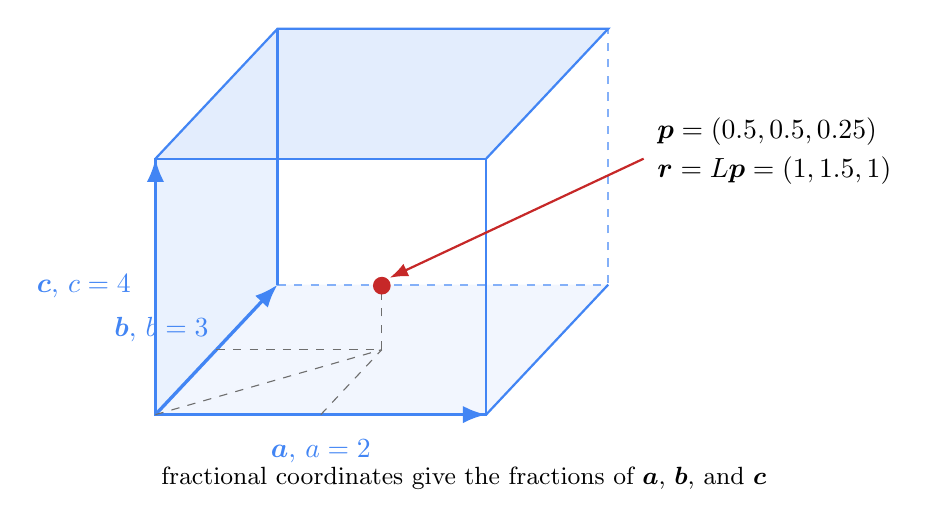
\begin{tikzpicture}[
  >=Latex,
  edge/.style={cellblue, thick},
  hidden edge/.style={cellblue!65, thick, dashed},
  lattice vector/.style={->, very thick, cellblue},
  guide/.style={guidegray, dashed, thin},
  label/.style={font=\small}
]

% Axonometric projection of the orthorhombic cell.
\coordinate (O)   at (0,0);
\coordinate (A)   at (4.2,0);
\coordinate (B)   at (1.55,1.65);
\coordinate (C)   at (0,3.25);
\coordinate (AB)  at ($(A)+(B)$);
\coordinate (AC)  at ($(A)+(C)$);
\coordinate (BC)  at ($(B)+(C)$);
\coordinate (ABC) at ($(A)+(B)+(C)$);

% Cell faces.
\fill[cellblue!7] (O) -- (A) -- (AB) -- (B) -- cycle;
\fill[cellblue!11] (O) -- (B) -- (BC) -- (C) -- cycle;
\fill[cellblue!15] (C) -- (AC) -- (ABC) -- (BC) -- cycle;

% Back and front edges.
\draw[hidden edge] (B) -- (AB) -- (ABC);
\draw[hidden edge] (B) -- (BC);
\draw[edge] (O) -- (A) -- (AC) -- (C) -- cycle;
\draw[edge] (C) -- (BC) -- (ABC) -- (AC);
\draw[edge] (A) -- (AB);
\draw[edge] (BC) -- (B);

% Lattice vectors from the origin.
\draw[lattice vector] (O) -- (A)
  node[midway, below=5pt] {$\boldsymbol a$, $a=2$};
\draw[lattice vector] (O) -- (B)
  node[midway, above left=-1pt] {$\boldsymbol b$, $b=3$};
\draw[lattice vector] (O) -- (C)
  node[midway, left=5pt] {$\boldsymbol c$, $c=4$};

% Fractional point p = 0.5 a + 0.5 b + 0.25 c.
\coordinate (Pa)  at ($(O)!0.5!(A)$);
\coordinate (Pab) at ($(Pa)+(0.5,0.0)$);
\coordinate (Pbase) at ($(O)!0.5!(A)+(O)!0.5!(B)$);
\coordinate (P) at ($(Pbase)+(0,0.8125)$);

\draw[guide] (O) -- (Pbase);
\draw[guide] (Pbase) -- (P);
\draw[guide] ($(O)!0.5!(A)$) -- (Pbase);
\draw[guide] ($(O)!0.5!(B)$) -- (Pbase);

\fill[pointred] (P) circle (3.2pt);
\draw[->, pointred, thick] (6.2,3.25) -- ($(P)+(0.10,0.10)$);
\node[align=left, anchor=west] at (6.25,3.35)
  {$\boldsymbol p=(0.5,0.5,0.25)$\\[2pt]
   $\boldsymbol r=L\boldsymbol p=(1,1.5,1)$};

\node[label, anchor=north west] at (-0.05,-0.55)
  {fractional coordinates give the fractions of $\boldsymbol a$, $\boldsymbol b$, and $\boldsymbol c$};

\end{tikzpicture}
\end{document}
